\begin{figure*}[!t]
    \centering
    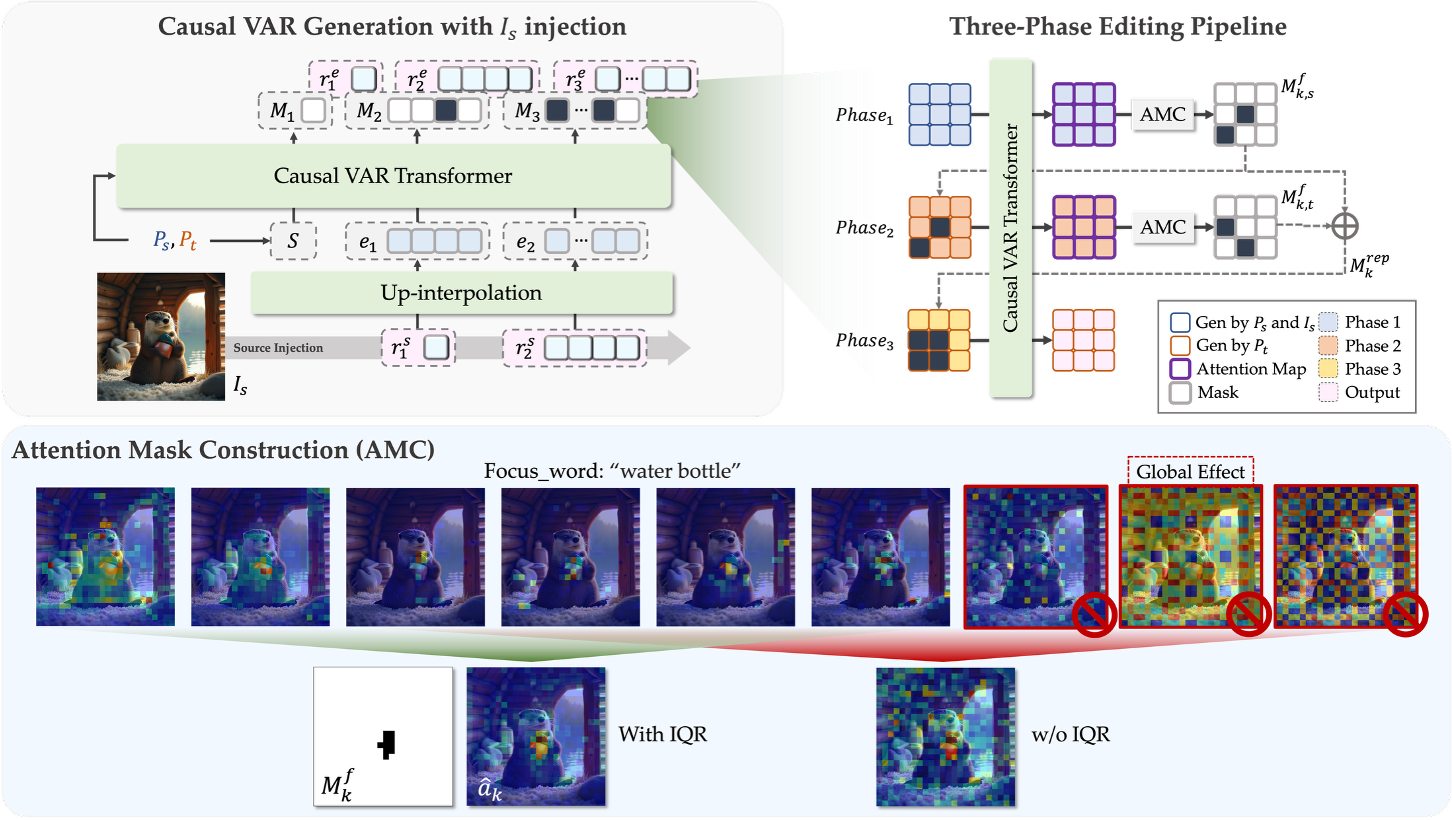
\includegraphics[width=\textwidth]{imgs/pipeline2.png}
    \caption{\textbf{Overview of the proposed editing framework.} \textit{Upper-left:} The source image $I_s$ is encoded into multi-scale discrete tokens $\{r_k^s\}$ via BSQ-VAE; for coarse scales ($k < N$), $r_k^s$ is directly injected into the causal VAR generation to preserve global layout. \textit{Upper-right:} For each scale $k \geq N$, three phases are executed: Phase~1 generates tokens conditioned on $P_s$ to extract $M_{k,s}^{\mathrm{f}}$ and $M_{k,s}^{\mathrm{p}}$; Phase~2 generates tokens conditioned on $P_t$ with background anchoring to extract $M_{k,t}^{\mathrm{f}}$; Phase~3 composes the final output by substituting background positions in $g_k$ with $r_k^s$ according to $M_k^{\mathrm{rep}} = \neg(M_{k,s}^{\mathrm{f}} \cup M_{k,t}^{\mathrm{f}})$. \textit{Bottom:} Detail of Attention Mask Construction (Sec.~\ref{sec:mask_construction}): per-block attention maps $a_{k,b}$ are filtered via IQR to discard positional-bias-dominated transformer blocks, and the retained maps are averaged to produce $\hat{a}_k$, which is then binarized into $M_k^{\mathrm{f}}$ and $M_k^{\mathrm{p}}$.}
    \label{fig:pipeline}
\end{figure*}
